\chapter{Estado del Arte}

En este capítulo hablaremos, principalmente, de dos importantes aspectos. El primero es la situación de la industria del entretenimiento digital hoy en día, seguido de una introducción a los videojuegos del género \textit{roguelike}. El segundo son los elementos que dificultan y facilitan el uso de diferentes programas y \textit{software} a ciertos sectores de la sociedad como invidentes o daltónicos; cómo algunos programas intentan solventar estos problemas y las razones por las que hemos elegido introducir ciertos elementos en nuestro proyecto para lidiar con los mismos.

\section{La industria del entretenimiento digital en la actualidad}

Desde sus primeros pasos hasta hoy en día, tal y como sucede con muchas de las novedades en el mundo del entretenimiento y la cultura, el sector del ocio digital ha sufrido cierto estigma por parte de una gran parte de la población, siendo censurado y degradado en mayor o menor medida, no tan solo por cierta parte de la sociedad al considerarlo como algo enfocado para niños y sin mucho interés o relevancia cultural, sino también por muchos medios de comunicación e incluso administraciones públicas. A pesar de que hoy en día este problema todavía está activo,\footnote{Es común que cada año en Australia se censuren algunos juegos como \href{http://goo.gl/hFrQah}{Paranautical Activity} por razones por las cuales otras formas de entretenimiento y cultura como películas o libros no se ven tan afectados \url{http://goo.gl/H2DXCW}} la industria se ha expandido tanto (consolas, ordenadores, navegadores, redes sociales, móvil...), que cada vez es más complicado encontrar a alguien que no haya jugado a algún videojuego en algún momento de su vida, ya que algo que forma parte del día a día de buena parte del público y defenderlo como un elemento de gran importancia cultural es cada vez más sencillo.

\subsection{La industria, en números}
En todo el mundo, pero especialmente en EEUU, la industria de los videojuegos es uno de los sectores con más crecimiento \cite{website:gamesimprovingeconomy} llegando a generar, solamente en ventas digitales, alrededor de 61 billones de dólares en el año 2015 \cite{website:gamingsales} y nuevos estudios comentan que no parará de crecer hasta el año 2019 \footnote{\url{http://goo.gl/yOlAzc}}. Ya en 2009 grandes títulos generaban más beneficios que las grandes producciones de \textit{Hollywood} \footnote{\url{https://goo.gl/yu3B4O}} y esta diferencia no ha hecho más que crecer desde entonces. En el año 2013 la industria cinematográfica americana ingresó globalmente 35.9 millones de dólares \footnote{\url{http://goo.gl/2A44Xk}}, mientras que la industria del entretenimiento digital en el mismo periodo ingresó 70.9 billones \footnote{\url{https://goo.gl/6avRXf}} y no ha hecho más que crecer desde entonces. En comparación con la industria musical, solamente el videojuego Grand Theft Auto V prácticamente generó el mismo número de beneficios. \footnote{\url{http://goo.gl/E79c68}}

Este gran éxito se debe, en gran parte, a la irrupción de los juegos desarrollados para dispositivos móviles, cuyo beneficio ha ido aumentando enormemente durante los últimos años. \footnote{\href{https://goo.gl/cvqds0}{La venta de videojuegos a nivel global crece año tras año, pero el mayor aumento de beneficio se está centrando en el mercado de los juegos para móvil.}} Sin embargo, esto no significa que el resto de plataformas no estén triunfando o se hayan quedado estancadas. Solamente Steam,\footnote{\url{store.steampowered.com}} la plataforma de distribución digital para PC por excelencia que ha sido desarrollada por Valve, ha generado alrededor de 3 billones y medio de dólares en el año 2015 \cite{website:steamgamesmarket}.

También hemos visto nuevas consolas salir al mercado hace poco más de dos años: PlayStation 4 y Xbox One. La primera de ellas ha logrado vender, a principios del año 2016, alrededor de 36 millones de unidades \cite{website:ps4sales}, mientras que la consola de Microsoft llega a los 19.1 millones en el mismo periodo \cite{website:xboxonesales}, haciendo un total de más de 55 millones de unidades en total, la cual es una gran cifra en comparación con los años anteriores.

Con el mercado del PC resurgiendo, las consolas de sobremesa obteniendo grandes cifras de ventas, las portátiles resistiendo la lucha contra los móviles, el mercado de los videojuegos para móvil en esplendor y los cascos de realidad virtual llegando al mercado este año 2016 y obteniendo grandes números de ventas y preventas, todo parece indicar que la industria de ocio digital no hará más que crecer durante los próximos años.

\subsection{Conclusión}

Lo que comenzó hace varias décadas como un modo de entretenimiento minoritario, generalmente enfocado a un público infantil o adolescente y que miraba a otras industrias como la cinematográfica con recelo, tanto en números como en visibilidad, se ha convertido en todo lo que había deseado y más. Gracias a grandes títulos y a su expansión a toda clase de dispositivos, no se puede hablar de la industria del entretenimiento sin hablar de videojuegos y, en muchos casos, algunos de esos títulos han logrado ser nombrados como obras de arte en su género, pasando a la historia y siendo recordados a lo largo de los años.
De hecho, varios museos, como el Museum of Modern Art (MoMA), están creando colecciones permanentes de videojuegos \footnote{\url{https://goo.gl/nioYtu}}.

\section{El género \textit{Roguelike.}}
\label{sec:roguelikeinformacion}

\subsection{Qué es y orígenes}

En 1983, Michael Toy y Glenn Wichman crearon un videojuego llamado \textit{Rogue},\footnote{Desde 2014 este juego se encuentra disponible en su totalidad y completamente gratuito en \href{https://archive.org/details/msdos_Rogue_1983}{archive.org}} que acabó definiendo el género \textit{roguelike}, el cual sigue vigente y gozando de gran esplendor hoy en día. Principalmente se centra en el control de un personaje que avanza por diferentes tipos de mazmorras derrotando enemigos, consiguiendo mejores estadísticas personales y objetos que permiten al usuario seguir avanzando. Se puede observar en la Figura \ref{fig:roguegame}.

Las características principales que definieron inicialmente a \textit{Rogue} y, por extensión, al género son:

\paragraph{\textit{Permadeath:}} Se trata de videojuegos con un nivel de dificultad destacado y caracterizados por lo que se denomina\textit{permadeath}. Una vez que el jugador muere, tiene que empezar desde el principio; no hay partidas guardadas (por lo que no puedes volver a atrás), aunque suele permitirse jugarse una misma partida en diferentes sesiones. Esta dificultad obligará al jugador a rejugarlo una y otra vez.

\paragraph{Aleatoriedad:} Cada vez que el jugador comienza una nueva partida se encontrará con ciertos elementos que han cambiado con respecto a la vez anterior: el mapa es distinto, los elementos y enemigos se encuentran en sitios diferentes, los objetos obtenidos han cambiado, etc., lo que favorece la rejugabilidad.

\paragraph{Progresión:} Una de las frases más escuchadas en las críticas positivas que \textit{Rogue} recibió tras su lanzamiento era que el jugador sentía la necesidad de intentar llegar más lejos en cada una de las partidas jugadas \cite{website:machinesnetworks}. Esto viene dado, sobre todo, por la sensación de progresión y de que en cada \textit{run}\footnote{Palabra comúnmente usada en estos géneros y que se refiere a una partida desde su inicio hasta que el jugador pierde} el usuario vaya mejorando. Dentro de la propia partida también existe una progresión a medida que el usuario derrota enemigos, consiguiendo puntos de experiencia, mejorando su personaje y equipamiento. La intriga por saber los nuevos objetos que se pueden conseguir, los nuevos enemigos con los que nos enfrentaremos y mapas que se generarán y explorarán, hace que el juego sea fácilmente rejugable y atrayente para todo tipo de usuarios.

\begin{figure}[h!]
		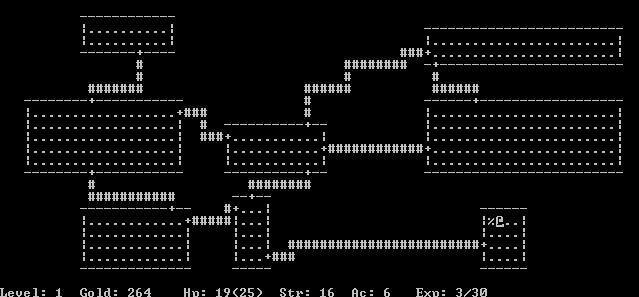
\includegraphics[width=\textwidth,height=\textheight,keepaspectratio]{./img/roguegame.PNG}
	\caption{Captura de pantalla del videojuego \textit{Rogue} con gráficos ASCII que describen el mapa y los elementos en él, muy usados en muchos \textit{roguelikes}, incluso hoy en día.}
	\label{fig:roguegame}
\end{figure}

A partir de este momento muchos fueron los títulos, algunos de ellos desarrollados por aficionados, que decidieron imitar estas características que hemos mencionado y añadiendo, cambiando o enfatizando diferentes elementos. Por este motivo es por lo que se denominan \textit{roguelikes}, dado que siguen los pasos marcados por \textit{Rogue}.
Por ejemplo, \textit{Rogue Legacy} \footnote{\url{roguelegacy.com}} tiene todos los elementos que hemos comentado, pero su combate en vez de ser por turnos es en tiempo real y la progesión viene dada a la hora de elegir el personaje a jugar y los objetos con los que equiparse en cada una de las partidas.

\subsection{En la actualidad}

Tras el éxito de \textit{Rogue}, fueron muchos los juegos que simularon su fórmula de éxito e intentaron mejorarlo, sobre todo gráficamente. Algunos se centran en diferentes aspectos (combate en vez de exploración, por ejemplo) y llegan a ser completamente diferentes a la hora de jugarlos (por turnos o tiempo real) pero, sin embargo, todos conservan buena parte de las características que hicieron al género famoso hasta hoy en día. Uno de ellos fue Vultures. Figura \ref{fig:vulturesgame}. 

\begin{figure}[h!]
		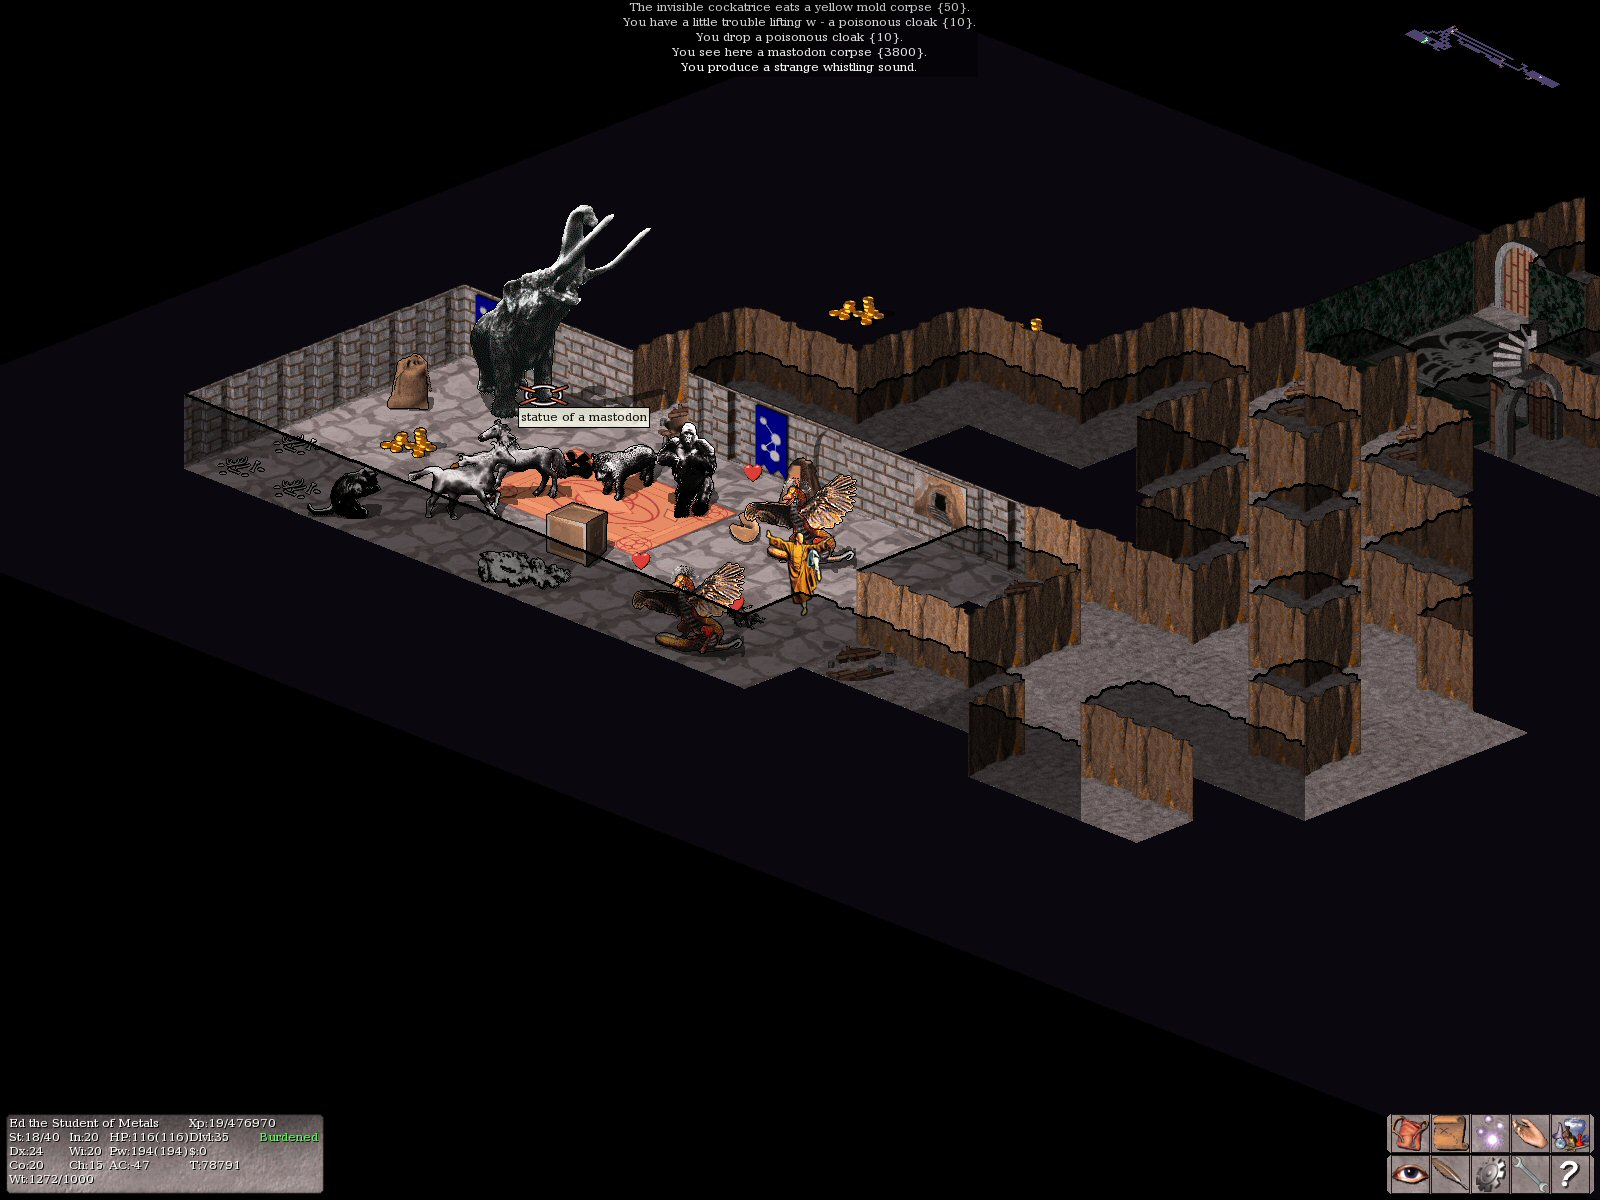
\includegraphics[width=\textwidth,height=\textheight,keepaspectratio]{./img/Vultures.jpg}
	\caption{Captura de pantalla del videojuego Vultures}
	\label{fig:vulturesgame}
\end{figure}

Incluso en la actualidad una gran cantidad de nuevos títulos, muchos de ellos desarrollados por empresas independientes, no dan especial importancia a tener gráficos realistas en tres dimensiones o texturas increíbles (por ello sigue habiendo muchos títulos con pseudo-gráficos en \textit{ASCII}), sino que optan por profundizar en crear una ambientación interesante y ofrecer un sistema de combate y exploración únicos y pulidos.
Uno de estos títulos que ha triunfado enormemente desde su lanzamiento en 2012, con más de dos millones de copias vendidas solamente en Steam,\footnote{\url{http://goo.gl/ZqrYbs}} es \textit{FTL: Faster Than Light}, del que hemos adjuntado una captura de pantalla en la Figura \ref{fig:ftl}, aunque no está considerado un roguelike al 100\%. ADOM,\footnote{\url{http://goo.gl/XHcVQ9}} sin embargo, que es un \textit{roguelike} a la vieja usanza, fue un proyecto de \textit{crowdfunding} que consiguió alrededor de cien mil dólares por parte de la comunidad y actualmente se vende en \textit{Steam}.

El género \textit{roguelike} también ha influido otros géneros como los \textit{action RPGs} y sagas como \textit{Diablo}\footnote{\url{us.battle.net/d3/en}}, que goza de millones de jugadores.
Elementos como el mencionado \textit{permadeath} o la generación procedural de mapas y misiones se han incluido en muchos títulos para hacerlos más atractivos, por ejemplo \textit{X-COM 2} \footnote{\url{https://xcom.com}} o el futuro y muy esperado \textit{No Man's Sky}, donde todo el universo y todos sus elementos son generados proceduralmente.\footnote{\url{http://goo.gl/ESoiml}}

\begin{figure}[h!]
		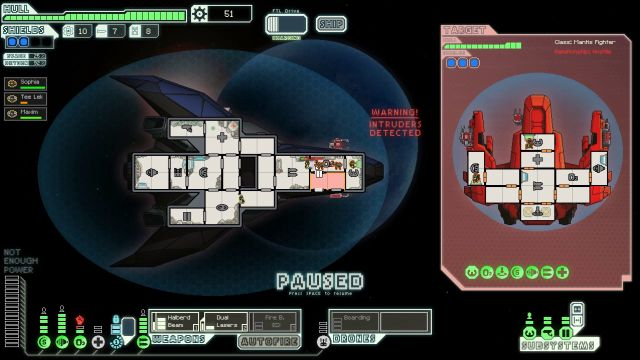
\includegraphics[width=\textwidth,height=\textheight,keepaspectratio]{./img/ftl.jpg}
	\caption{Captura de pantalla del videojuego FTL: Faster Than Light}
	\label{fig:ftl}
\end{figure}

\subsubsection{La aparición de subgéneros}

Perder todo el progreso y tener que empezar desde el principio sin haber conseguido nada más que la experiencia personal es algo que no atrae al perfil del jugador actual (con una media de edad que no puede permitirse cientos de horas jugando). Por esta razón son numerosos los juegos que han añadido más elementos de progreso general para que el jugador no se sienta frustrado y consiga una recompensa de forma más inmediata. Estos incentivos pueden ser nuevos personajes con los que jugar, puntos de experiencia generales o dinero con lo que poder equipar y mejorar desde un principio a nuestro personaje para poder llegar más lejos que la anterior vez, diferentes modos de juegos que se desbloquean al llegar a una cierta puntuación, etc.
También es más común ver juegos de este tipo que se basan en partidas cortas, de como mucho una hora, para que la repetición sea mayor y perder el personaje no se vea como un fracaso, sino algo que forma parte del juego en sí.

Estos cambios han modificado el género que \textit{Rogue} creó en un inicio y no siempre se han tomado positivamente por parte de la comunidad de aficionados más conservadores, que se suele quejar de que muchos títulos que se definen a sí mismos como \textit{roguelike} no contienen ciertas características, que una vez definieron el género, especialmente en tema de dificultad. Por este motivo se han definido subgéneros como el \textit{roguelite}, que toman muchas de esas ideas iniciales, pero añaden o ignoran otras muchas para crear un título que sea un poco más sencillo y no penalice tanto al jugador. Algunos títulos de este género son \textit{Binding of Isaac}\footnote{\url{bindingofisaac.com}} o \textit{Ziggurat}\footnote{\url{http://goo.gl/wB1kCU}}.

Debido a estos nuevos subgéneros, se han creado definiciones que miden el nivel de \textit{roguelike} que tiene un título. Una de ellas es llamada ``Berlin interpretation''. \footnote{\url{http://goo.gl/29nDSp}}

\subsection{Elementos \textit{roguelike} en nuestro proyecto}

En nuestro caso hemos creado un \textit{roguelike} de corte más purista, similar a Rogue, no solamente estéticamente, pero también en diseño y funcionalidad. El jugador explorará un mapa aleatoriamente generado y luchará contra diferentes enemigos que intentarán eliminarlo de diferentes formas. En base al nivel que el usuario tenga, los enemigos serán más o menos poderosos y la recompensa por abatirlos será mayor.

El objetivo del juego es llegar lo más lejos posible dentro de la mazmorra. Cada vez que el jugador entre en un portal se incrementará su puntuación (el número de puntos se mostrará en la pantalla) y, cada vez que esto suceda, un nuevo mapa será generado con diferentes características y contenido, por lo que el jugador tendrá que volver a buscar la salida de este nuevo nivel, batiendo enemigos, descubriendo tesoros, y mejorando sus estadísticas personales durante dicho recorrido. El juego es complicado, aleatorio y con una sensación de progreso, tal y como corresponde al género \textit{roguelike}.

%\begin{figure}[H]
%		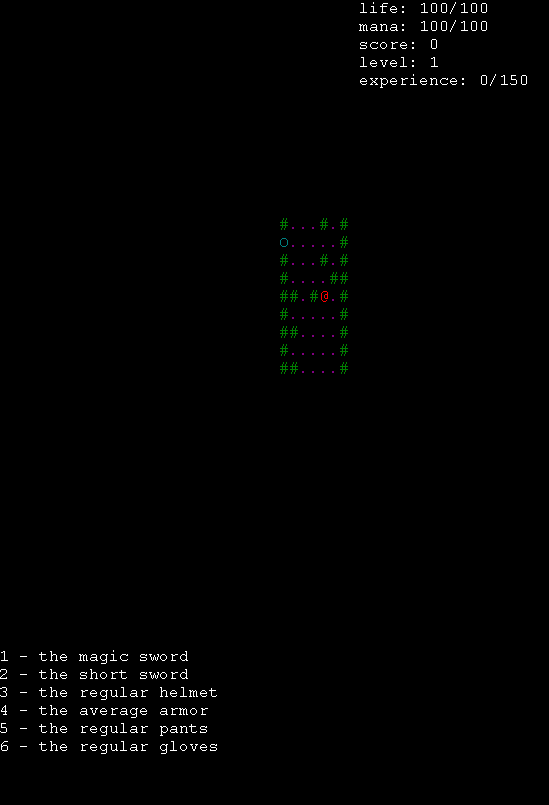
\includegraphics[width=140mm, height=185mm]{./img/roomsGameGeneral.png}
%	\caption{Captura de pantalla de la interfaz de usuario de nuestro juego}
%	\label{fig:roomsgamegeneral}
%\end{figure}

\section{Problemas de la tecnología para invidentes y daltónicos}
\label{sec:dificultadesfeedback}

Algunos de los factores que hacen de la tecnología un elemento prácticamente imprescindible hoy en día y que facilitan su usabilidad crean, paradójicamente, una barrera para mucha gente que no puede disfrutar de ella, dificultando su día a día enormemente.

En esta sección hablaremos sobre algunos de los problemas que tanto invidentes como daltónicos se encuentran actualmente a la hora de usar diferentes tipos de software (especialmente videojuegos). Asimismo veremos cómo, en bastantes ocasiones, solventarlos no requiere nada más que prestar un poco de atención y tener en cuenta aspectos simples, lo que pone en manifiesto que muchas de estas limitaciones son dadas más por el desconocimiento que por la dificultad o coste de implementar una solución.

\subsection{Dificultades a las que se enfrentan los invidentes}

A pesar de que han sido muchos los avances que hemos podido observar durante los últimos años en esta área, las dificultades que tienen invidentes o personas con diferentes grados de ceguera en nuestra sociedad son enorme y, tristemente, tanto dispositivos tecnológicos como \textit{software} no se ven excluidos de esta lista.
No poder hacer uso de una interfaz gráfica o ver lo que está sucediendo en la pantalla es un problema que automáticamente imposibilita el uso de la mayoría de las aplicaciones y videojuegos. Incluso navegar por Internet, donde la mayoría del contenido es texto que debería poder ser leído fácilmente por un lector de pantalla, puede llegar a ser un quebradero de cabeza.

\subsection{Cómo abordar parte de estos problemas para los invidentes}

Uno de los principales problemas de los que se quejan los usuarios, tal y como nos señalaron los informadores en la charla de la \textit{ONCE}, es que muchos de los desarrolladores de software o adaptaciones específicas para ciegos no tienen en cuenta que, la mayoría de las veces, junto al usuario invidente hay también usuarios videntes que les pueden describir lo que está sucediendo en la pantalla. Por ello es muy importante crear una interfaz que esté actualizada y muestre la misma información que la persona invidente reciba.

En el caso de los videojuegos, algunos de ellos han visto versiones adaptadas para invidentes, la mayoría de ellas creadas por la propia comunidad y no por las empresas desarrolladoras, así como nuevos títulos que se centran en ofrecer una experiencia revolucionaria desde el principio. Un buen ejemplo de ello es Shades of Doom,\footnote{\url{http://www.gmagames.com/sod.html}} que solamente usa sonido (principalmente ruidos repetitivos) y muy pocas frases para que el jugador sea capaz de descubrir lo que tiene que hacer, dónde está dentro del mapa, y describir todos los elementos que un usuario vidente recibe a través del uso de una interfaz gráfica.

También existen juegos originales que están completamente adaptados para invidentes, como es el caso de \textit{A Blind Legend}\footnote{\url{https://goo.gl/nasbIx}} para \textit{Android}.

\subsection{Tiflotecnología}

La tiflotecnología es el conjunto de técnicas, conocimientos y recursos enfocados a ayudar a personas con cualquier tipo de deficiencia visual para que puedan usar dispositivos electrónicos fácilmente.
Ejemplos de tiflotecnología serían lupas magnificadores, tanto a nivel de \textit{software} como \textit{hardware}; \textit{software} de lectura de pantalla como \textit{NVDA}, o barras de braille que permiten al usuario leer lo que está en la pantalla y que suele ser usada para diferentes tareas como programar o realizar cálculos matemáticos.

En nuestro proyecto hemos tenido en cuenta estos elementos para adaptar lo mejor posible nuestro juego a las herramientas que las personas con deficiencia visual usan en su día a día.

\subsection{Dificultades a los que se enfrentan los daltónicos}

El daltonismo es un defecto genético que afecta aproximadamente al 1\% de la población y que tiene diferentes variantes dependiendo de los tipos de colores con los que tienen problema. Lo que en un principio parece como un pequeño inconveniente que no debería afectar demasiado la vida de la persona que lo sufre, lo cierto es que hay muchas ocasiones en las que incluso disfrutar de un simple partido de fútbol puede convertirse en algo casi imposible para ellos, dado que en algunos partidos los jugadores llevan camisetas con colores problemáticos. \footnote{\url{http://goo.gl/o3GkrP}} Incluso ver un mero mapa puede ser una complicación\footnote{\href{https://i.imgur.com/CMCywUU.jpg}{Imagen que muestra los diferentes tipos de daltonismo y cómo lo perciben personas con diferentes tipos de daltonismo}}.

En el caso de los videojuegos, donde los gráficos y paletas de colores juegan un gran papel en el arte del título, este problema se ve acentuado, especialmente si parte de las mecánicas del juego necesitan que el jugador sea capaz de distinguir colores para obtener cierta información relevante, y esto es algo que sucede en numerosos títulos. En algunos casos puede suponer una pequeña molestia como en \textit{Borderlands},\footnote{\url{www.borderlandsthegame.com}} un juego de acción en primera persona donde hay armas especiales que se diferencian, únicamente, por el color en el que se encuentra un determinado texto. En la Figura \ref{fig:borderlandsnormal} se puede observar cómo se vería normalmente y en la Figura \ref{fig:borderlandscolorblind} cómo algunas personas daltónicas lo ven. 
Sin embargo, el mayor problema viene cuando estas limitaciones pueden llegar a arruinar el juego, como ocurre en \textit{The Witness},\footnote{\url{http://goo.gl/GYPdhH}} un juego de puzzles ya mencionado en apartados anteriores en el que, para poder resolver muchos de ellos, es preciso que el usuario pueda distinguir distintos colores. 
También nos encontramos con juegos de lucha en dos dimensiones donde la única diferencia entre los escenarios del fondo y los personajes principales es el color de los mismos. No ver la diferencia complica que el jugador detecte si un elemento está al frente o al fondo de dicho escenario.

\begin{figure}[H]
		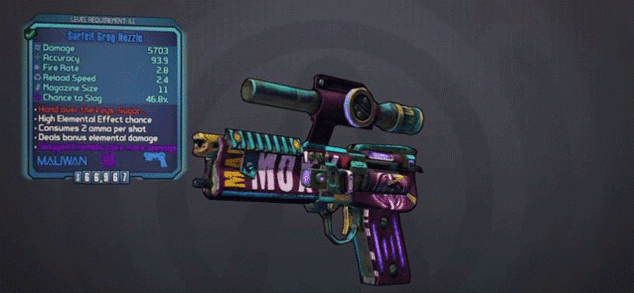
\includegraphics[width=\textwidth,height=\textheight,keepaspectratio]{./img/borderlandsnormal.png}
	\caption{Captura de pantalla del juego Borderlands para personas sin daltonismo.}
	\label{fig:borderlandsnormal}
\end{figure}

\begin{figure}[H]
		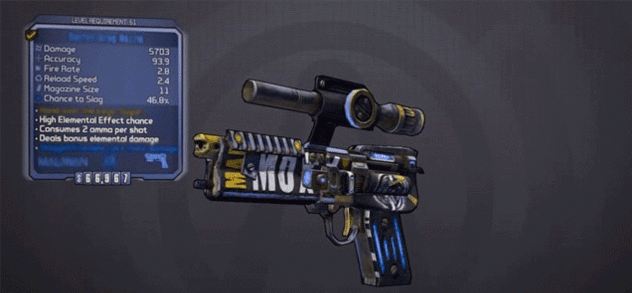
\includegraphics[width=\textwidth,height=\textheight,keepaspectratio]{./img/borderlandscolorblind.png}
	\caption{Captura de pantalla del juego Borderlands para personas con cierto tipo de daltonismo.}
	\label{fig:borderlandscolorblind}
\end{figure}

\subsection{Cómo abordar parte de estos problemas para los daltónicos}
\label{sec:daltonicossolventar}

Para poder dar respuesta a esta cuestión, y debido a su naturaleza, se creyó conveniente informarse respecto a la misma de mano de los propios afectados. En nuetro caso recurrimos al portal \textit{Reddit} para consultar a los usuarios daltónicos sobre cómo desarrollar un juego que sea adecuado para ellos \footnote{\url{https://goo.gl/d6cTqe}}. Fueron muchas las respuestas obtenidas, pero se puede resumir en dos alternativas.

La primera es que, en la medida de lo posible, nunca tengamos que diferenciar dos elementos distintos únicamente por su color. A modo de ejemplo y, tal y como un usuario comentó, si estamos desarrollando un juego tipo ``Hundir la Flota'' y la diferencia entre un barco intacto y uno averiado es que cambiamos su color de verde a rojo, también deberíamos de añadir llamas u otros elementos distintivos a mayores que faciliten al usuario apreciar visualmente que se ha producido un cambio. Del mismo modo, si tenemos un juego tipo \textit{Tetris} o \textit{Candy Crush} donde las piezas son relevantes, en vez de distinguirlas sólo por su color, podríamos hacerlas de formas diferentes o añadir una imagen a cada una de ellas.

La segunda opción es que, si fuese completamente necesario emplear únicamente diferentes colores para diferenciar ciertos elementos entonces deberíamos, o bien optar por combinaciones de colores que, generalmente, no creen ningún problema (azul, amarillo, verde...) lo cual tampoco nos garantiza que hayamos solventado el problema dado que, como ya hemos comentado, hay muchas formas de daltonismo y en algunas de ellas el usuario todavía puede tener problema diferenciándolos dependiendo del color contreto usado), o bien añadimos una opción mediante la que podamos cambiar la paleta de colores usada. Hay algunos videojuegos, la mayor parte de ellos independientes, donde se da esta última opción. 